\subsubsection{jExam Launcher}

jExam Launcher ist der Hauptdienst von jExam. Er ist für die Ausführung
und Bereitstellung von \Gls{jexam_new} und \Gls{jexam_2009} zuständig. Der Dienst
besteht aus fünf Containern, darunter :

\begin{itemize}
    \setlength\itemsep{1em}

    \item[] \textbf{JBoss}: Dieser Container enthält das Skript zum
    Bereitstellen des JBoss-Servers, den \Gls{jexam_new} und \Gls{jexam_2009}
    benötigen, um funktionieren zu können. Dieser Server dient auch
    als Datenbank für die beiden Apps. Er legt daher einige seiner
    Ports offen, um für externe Verbindungen zugänglich und offen
    zu sein.

    \item[] \textbf{Initializer}: Dieser Container enthält ein
    Java Skript, das automatisch (oder auf Wunsch des Testers auch
    manuell) ausgeführt wird und dazu dient, Testdaten in den 
    JBoss-Server zu injizieren. Es initialisiert die Daten, die für
    die Ausführung der Tests erforderlich sind.

    \item[] \textbf{OldWeb}: Dieser Container ermöglicht das
    Deployment von \Gls{jexam_2009}. Er enthält einen Tomcat-Webserver,
    der den Code von \Gls{jexam_2009} ausführt und sich dann mit
    dem Container verbindet, der den JBoss-Server enthält.
    Dieser Container legt ebenfalls seine Ports offen, damit er
    von den Tests erreicht werden kann, wenn diese im lokalen 
    Modus ausgeführt werden.

    \item[] \textbf{Webservice und Web}: Diese beiden Container
    ermöglichen die Ausführung und Bereitstellung von
    \Gls{jexam_new}. Der Webservice enthält eine API, die vor
    allem mit dem JBoss-Server kommuniziert. Der Web-Container
    enthält das Frontend der Anwendung. Web verbindet sich mit
    dem Webservice, wenn er gestartet wird, und stellt Ports zur
    Verfügung, die ihn zugänglich machen, wenn die Tests im
    lokalen Modus gestartet werden.
\end{itemize}

\begin{figure}[H]
    \centering
    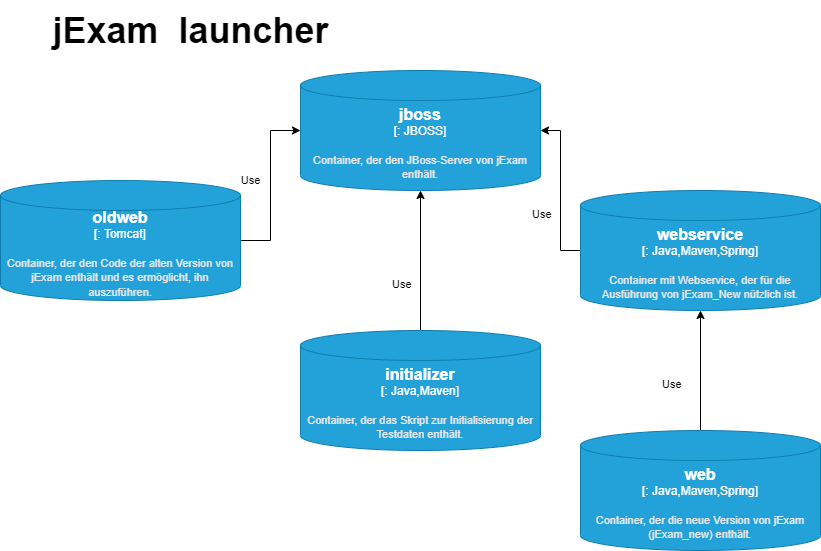
\includegraphics[scale=0.6]{images/launcher.drawio}
    \caption{JExam Launcher Testservice} \label{fig:laucher}
\end{figure}